\section*{Introduktion}
Formålet dette projekt er at illustrere relevante færdigheder, tilegnet på
snedkeruddannelsens grundforløb, KTS.
Projektet består af denne rapport samt billag, og det møbel rapporten omhandler.
Projektet omfatter blandt andet; design og arbejdstegning i CAD program
(\texttt{SolidWorks}), procesbeskrivelse, skæresedel, bestilling af råtræ uden
overdreven spild, behandling af råtræ, maskin- og hånd-lavede samlinger og finerarbejde.

Projektet er et natbord, inspireret af to lignende projekter fra
\texttt{CITYJOINERY}\nolinebreak \footnote{\texttt{cityjoinery.com}}.

\begin{figure}[htb]
\centering
\fbox{
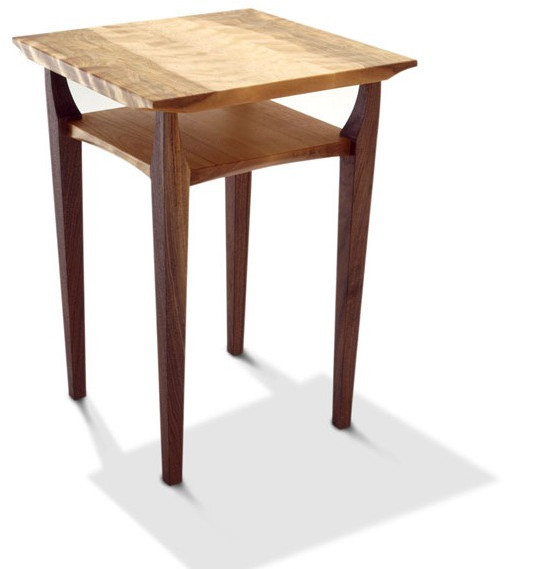
\includegraphics[width=0.4 \textwidth]{imgs/Aspiration-Nightstand-birch.jpg}
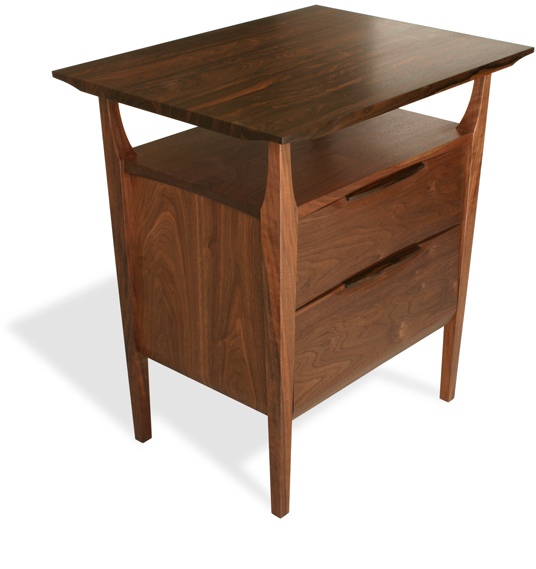
\includegraphics[width=0.4 \textwidth]{imgs/Aspiration-Nightstand-walnut.jpg}
}
\caption{Ende- og nat-bord fra \texttt{CITYJOINERY} i hhv. birk og valnød til
venstre, og valnød til højre.}
\end{figure}

\section*{Koncept \& Design}
Projektet er et fribensmøbel med sarge, én skuffe med hylde over,
og en bordplade. Ben, sarge og skuffe front udføres i massiv valnød,
skuffebund, hylde og bordplade, laves af birke-krydsfiner med
valnøddefiner og kantlister, skuffesiderne udføres i elm. Skuffen styres af
flere lister bag sargene, gjort i ahorn. Ben og sarge samles med maskinlavede
tap-slids samlinger. Skuffen laves med gennem-sinkede svalehalesamlinger, med
undtagelse af skuffefronten der laves fordækt.

\subsection*{Materialer}
Natbordets bordplade og hylde udføres i krydsfiner, da det er mere stabilt
end massivtræ. Da begge elementer fæstnes til benene, kan de potentielt
skævvride hele møblet, hvis de skulle slå sig med tiden. Brugen af finerede
pladematerialer løser det problem. Alternativt kunne man have brugt samlinger
der giver emnerne mulighed for at forskyde sig i forhold til hinanden, uden
større påvirkning på resten af møblet.

Valget af elm til skuffesiderne er kontroversielt. Traditionelt bruger man gerne
ahorn til skuffesider. Elm er kendt for at være splintret, med et ujævnt fiber
forløb, der kan virke sløvende på værktøjer, og let får oprifter\footnotemark. I
dette projekt bruges elm primært for sin æstetiske værdi, da kerneveddet kan
have en række forskellige farver (lilla og grønne strøg langs årene). Denne
æstetiske finurlighed vælges her fremfor den lettere arbejdsproces og større
farve kontrast ahorn havde givet (kontrast til skuffefronten i amerikansk
valnød). Det viser sig imidlertid at elm har flere glimrende egenskaber. Selvom
det har omtrent samme volumensvind ved tørring som ahorn ($\sim12\%$, mod ahorns
$\sim11\%$) er svindet tangentialt mindre, relativt til svindet radialt. Ahorn
har, ligesom egetræ, et tangentialsvind der er mere end dobbelt så stort som
radialsvindet. Uligheden mellem tangential- og radial-svind er den primære årsag
til at træ skælvrides når fugtigheden varieres. Hvis det radiale, tangentiale og
aksiale svind var det samme, ville træet blot variere i størrelse med
fugtigheden, uden at deformeres. En anden årsag til deformation kan være spændinger i træet, der
opstår når det vokser i blæst, eller på en skråning. Disse spændinger hjælper
til  at holde træet oprejst mens det gror, men når træet skæres op frigives
spændingerne, hvilket kan medføre \textit{stor} deformation.
Da stabilitet er ekstra vigtig i
skuffesiderne, er alt elmetræet skåret ned til spejlskårne stave, og
stavlimet. Ved opskæringen kan spændinger frigives, hvorefter stavene afrettes
og limes sammen. Som et kuriosum kan
det nævnes at indersiden af elmebark, i tider med hungersnød, har været brugt
som erstatning for mel i bagværk.

Mens skuffens elme-sider stavlimes, laves ben, sarge og skuffefront i massive
udskæringer af valnød. Dette kan (forhåbentligt) gå an uden for meget
deformation, da alle stykkerne er spejlskårne, og da valnød er hvad man kalder
en dimensionsstabil træsort. Med et tangentialt svind på $\sim 5\%$ mod et
radialt svind på $\sim7\%$

Det bør nævnes at kantlisterne er lavet i splintved, hvilket nedsætter møblets
levetid, især i friluft. Møblet bør derfor holdes indendørs, og olieringen
vedligeholdes. Da møblet bruger styrelister af ahorn, og skuffesider af elm,
ville det dog ikke alligevel være anbefalelsesværdigt at opbevare møblet udendørs,
og det ville i øvrigt fjollet da projektet er et natbord. Håbet er at det lyse
splintved kan tilføje en organisk dynamik til borpladens udseende, der kommer
til at have en overgang fra splintveddet i kanlisterne, til det mørkere
valnødefiner på borpladen og låget.

\footnotetext{Når andet ikke er angivet, er fakta om træsorter taget fra
\texttt{Træarter - TRÆ69}, fra \texttt{Træinformation}. ISBN 978-87-90856-328}

\subsection*{Udskæringer}
Natbordet har fået flere udskæringer og taperinger, der skal få det til at
fremstå mindre og lettere end det i virkeligheden er. Hvert ben er taperet på
begge ydersider, hvilket  efterlader indersiderne -- ind mod resten af møblet --
som lodrette plan der bruges som reference for skuffen og sargene. Modsat
taperingerne er toppen af benene bortfræset fra møblets inderside, hvilket giver
benenes taperede ydersider et øget blikfang. Det giver illusionen af at benene
er montereret skrånende på møblet, selvom indersiderne er lodrette. Det ønskes
at sargenes yderside i bunden flugter benenes, ligesom deres indersider er
koplanare med benenes indersider. Førstnævnte for visuel sammenhæng, sidstnævnte
for at skuffen kan styres af sargene, uden brug af styrelister. For at det kan
opnås, er sargene 34mm tykke, svarende til benenes tykkelse, målt 200mm fra
toppen.

For at mindske friktion, og risiko for skader, bør åreretningen på skuffens
bærelister gå langs skuffesiderne når skuffen skubbes ind. Det samme gælder
åreretningingen på skuffesiderne. Dette opnås nemt på bærelisterne i møblets
sider, men er mere problematisk for den bagerste og forreste bæreliste.
Problemet løses ved at høvle en smule af undersiden af skuffens bagside, så den
ikke kommer i kontakt i med bagerste bæreliste, og ligeledes ved at tage en
smule at begge ender på forreste bæreliste, hvis hovedformål alligevel er at
stabilisere de forreste ben, der ikke har en sarg imellem sig, samt at fungere
som et ekstra dybdestop for skuffen, så noget af slaget tages af den
bagerste sarg når skuffen lukkes.
